% 1270(본책 177쪽) — 평행한 가로 직선 4개와 세로 직선 6개가 간격 1로 수직으로 만나는 격자. 스캔 그림을 TikZ 로 다시 그림. 라벨 없음.
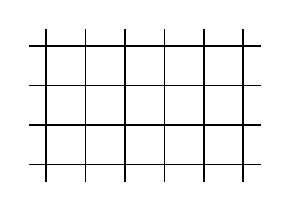
\begin{tikzpicture}[x=0.5cm, y=0.5cm, line width=0.6pt]
  \foreach \y in {0,1,2,3} { \draw (-0.45,\y) -- (5.45,\y); }
  \foreach \x in {0,1,2,3,4,5} { \draw (\x,-0.45) -- (\x,3.45); }
\end{tikzpicture}
